\begin{figure*}[t]
    \centering
 \begin{tabular}{cccccc}
   
    \multicolumn{6}{c}{%
        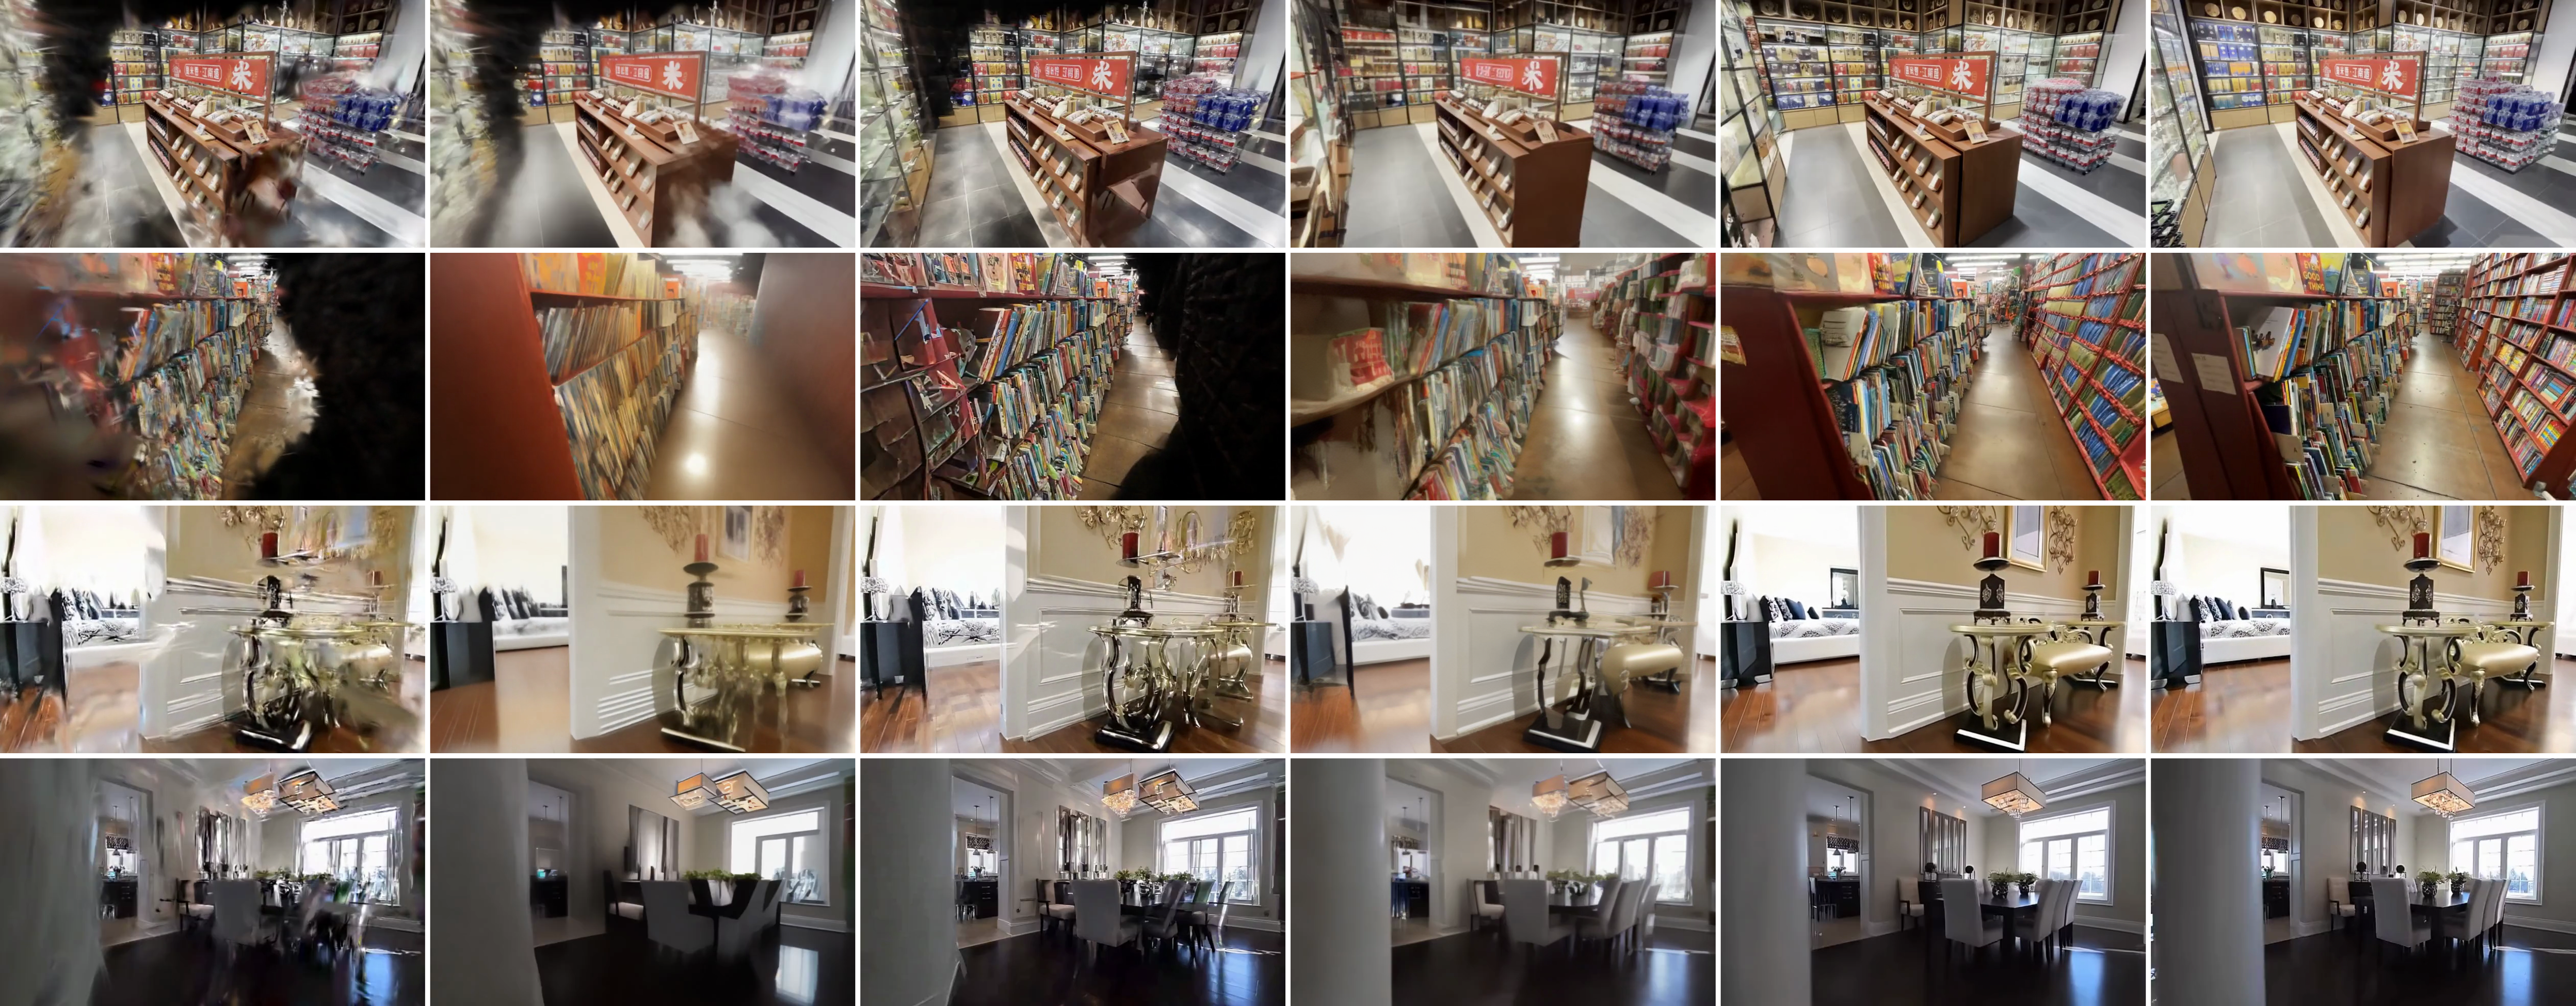
\includegraphics[width=\linewidth]{fig/image/main_comparison.png}%
    } \\
     \hspace{0.4cm} \small Splatfacto~\cite{ye2025gsplat} & 
    \hspace{0.4cm} \small GenFusion~\cite{Wu2025GenFusion} & 
    \hspace{.5cm}\small Difix3D+~\cite{wu2025difix3d} & 
    \hspace{.6cm}\small ExploreGS~\cite{Kim_2025_ExploreGS} &
    \hspace{0.2cm}\small \ours (Ours) & 
    \hspace{-0.1cm}\small Ground Truth \\
    \midrule
    \multicolumn{6}{c}{%
        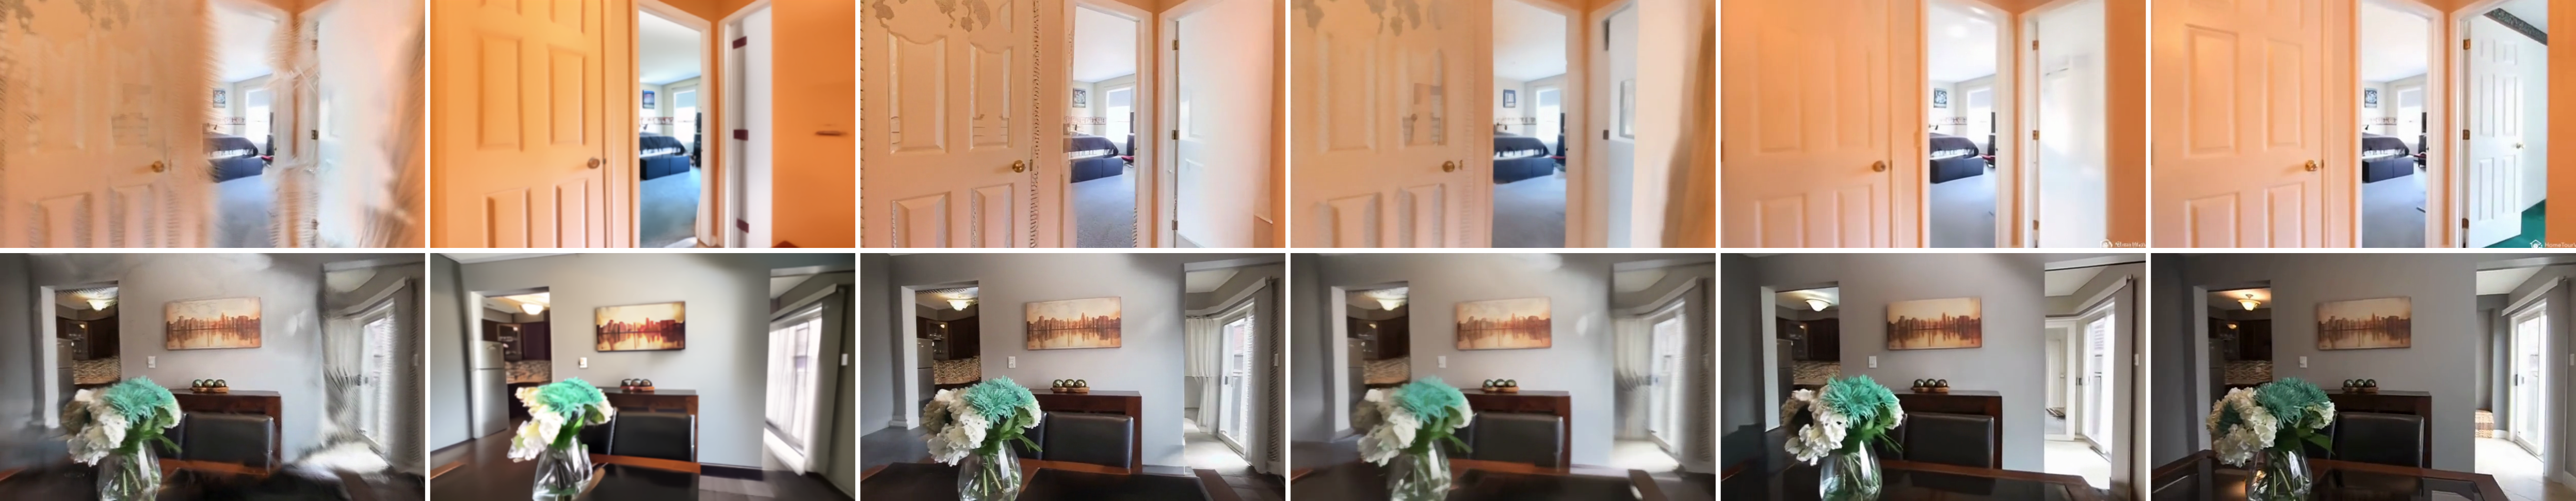
\includegraphics[width=\linewidth]{fig/image/main_comparison_part2.png}%
    } \\
    \hspace{0.4cm} \small DepthSplat~\cite{xu2024depthsplat} & 
    \hspace{0.4cm} \small MVSplat360~\cite{chen2024mvsplat360} & 
    \hspace{.5cm}\small Difix3D+~\cite{wu2025difix3d} & 
    \hspace{.6cm}\small ExploreGS~\cite{Kim_2025_ExploreGS} &
    \hspace{0.2cm}\small \ours (Ours) & 
    \hspace{-0.1cm}\small Ground Truth \\

\end{tabular}  
   \caption{\textbf{Qualitative Comparison on Novel-View Refinement.}
We compare \ours with baseline methods on diverse scenes from DL3DV~\cite{ling2024dl3dv} and RE10K~\cite{re10k}. 
\ours effectively removes rendering artifacts such as blur, floaters, ghosting, and texture distortions, producing sharper geometry, cleaner reconstruction than Splatfacto~\cite{ye2025gsplat}, GenFusion~\cite{Wu2025GenFusion}, DiFiX3D+~\cite{wu2025difix3d}, and ExploreGS~\cite{Kim_2025_ExploreGS}, and achieving visual fidelity closest to the ground truth. 
From top to bottom, our model demonstrates strong generalization across various refinement scenarios: (\textit{1}) inpainting missing regions, (\textit{2}) outpainting beyond the original view, (\textit{3–4}) correcting blur, ghosting, and geometric errors, and (\textit{5–6}) handling artifacts from feed-forward 3DGS models, including transparent Gaussian primitives and spiky geometry. 
% While baselines handle certain artifact types, they fail to generalize as robustly as \ours.
}

    \label{fig:image_refine}
\end{figure*}


% \begin{figure*}[t]
%     \centering
%     \setlength{\tabcolsep}{3pt} % tighten columns a bit
%     \renewcommand{\arraystretch}{1.0}
%     \begin{tabular}{@{}p{1.6cm}cccccc@{}} % <-- left label column
%         % -------- TOP BLOCK (4 rows inside the image) --------
%         \multirow{1}{*}{\centering
%             \rotatebox{90}{\parbox{3.2cm}{\centering \small Optimization-based\\[-2pt] 3DGS}}
%         }
%         & \multicolumn{6}{c}{%
%             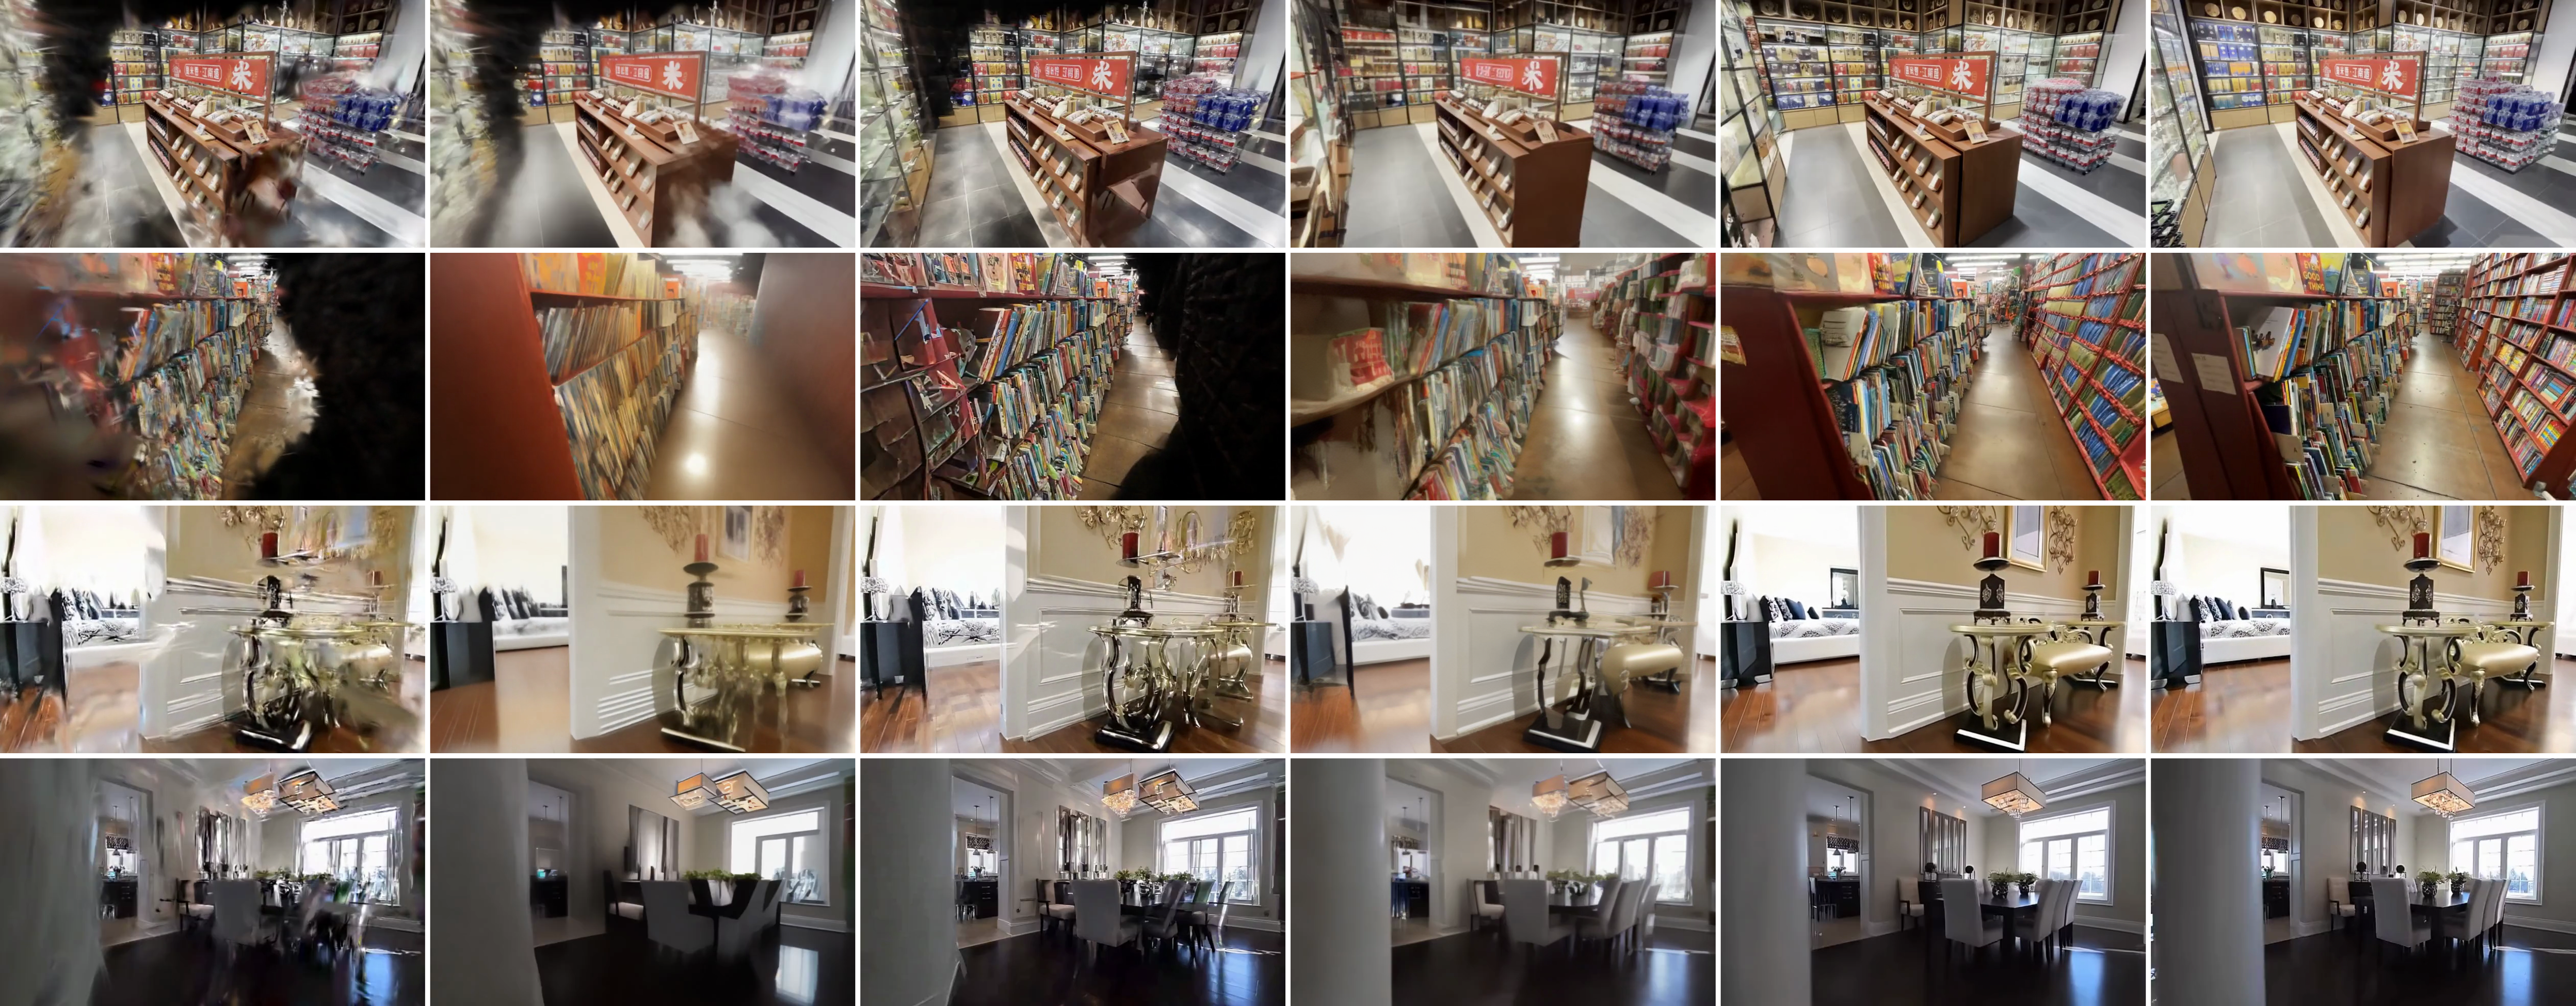
\includegraphics[width=\linewidth]{fig/image/main_comparison.png}%
%         } \\
%         & \hspace{0.4cm} \small Splafacto~\cite{ye2025gsplat} &
%           \hspace{0.4cm} \small GenFusion~\cite{Wu2025GenFusion} &
%           \hspace{.5cm}\small Difix3D+~\cite{wu2025difix3d} &
%           \hspace{.6cm}\small ExploreGS~\cite{Kim_2025_ExploreGS} &
%           \hspace{0.2cm}\small \ours (Ours) &
%           \hspace{-0.1cm}\small Ground Truth \\
%         \midrule
%         % -------- BOTTOM BLOCK (2 rows inside the image) --------
%         \multirow{2}{*}{\centering
%             \rotatebox{90}{\parbox{3.2cm}{\centering \small Feed-forward\\[-2pt] 3DGS}}
%         }
%         & \multicolumn{6}{c}{%
%             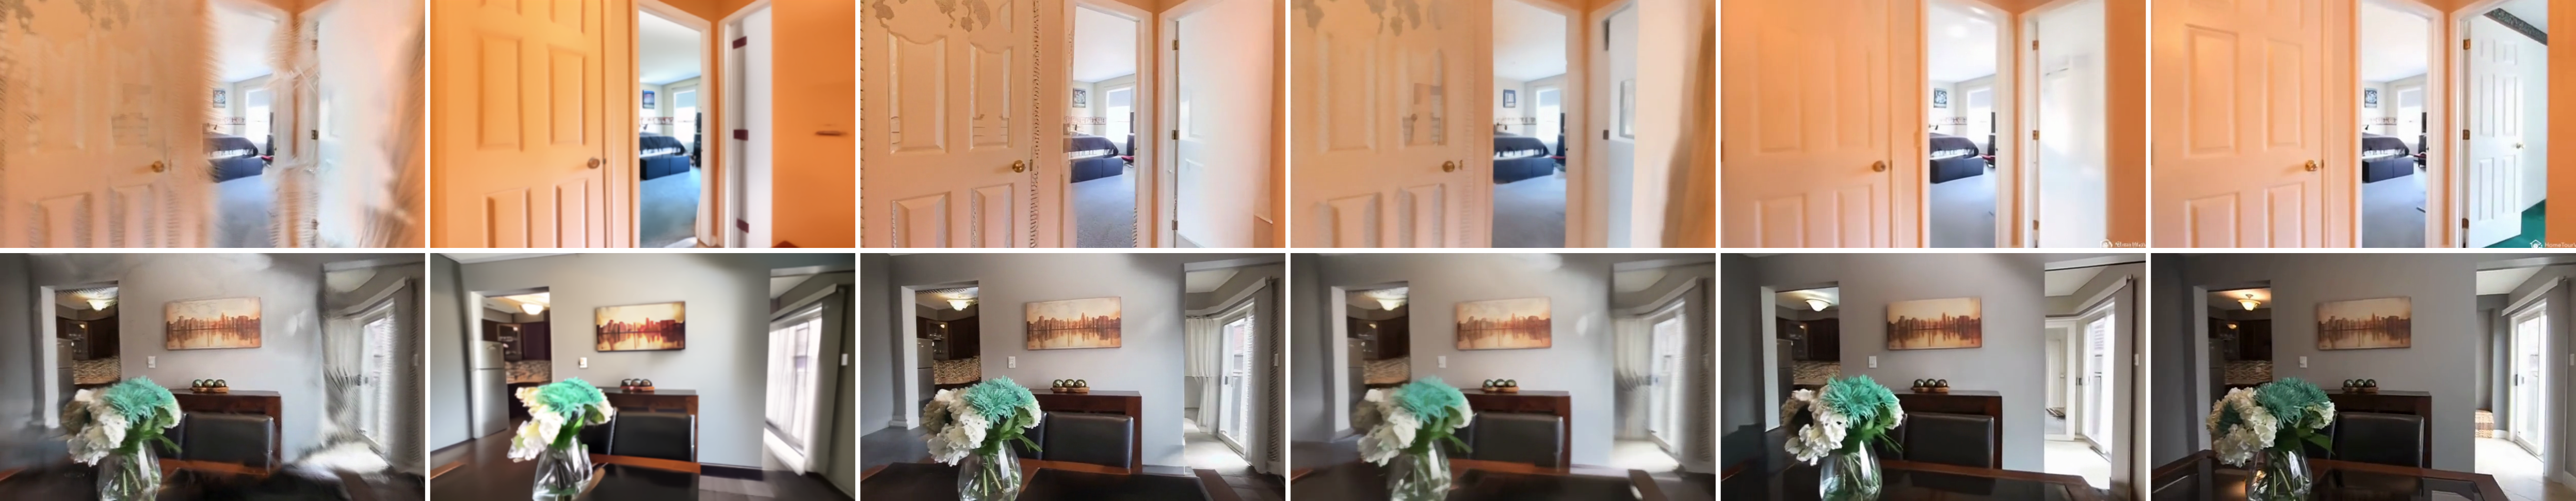
\includegraphics[width=\linewidth]{fig/image/main_comparison_part2.png}%
%         } \\
%         & \hspace{0.4cm} \small DepthSplat~\cite{xu2024depthsplat} &
%           \hspace{0.4cm} \small GenFusion~\cite{Wu2025GenFusion} &
%           \hspace{.5cm}\small Difix3D+~\cite{wu2025difix3d} &
%           \hspace{.6cm}\small ExploreGS~\cite{Kim_2025_ExploreGS} &
%           \hspace{0.2cm}\small \ours (Ours) &
%           \hspace{-0.1cm}\small Ground Truth \\
%     \end{tabular}
%     \caption{\textbf{Qualitative Comparison on Novel-View Refinement.} ...}
%     \label{fig:image_refine}
% \end{figure*}
